\documentclass[10pt]{article}
\usepackage{titling}
\usepackage{lipsum}
\usepackage{amsmath}
\usepackage{listings}
\usepackage{graphicx}
\usepackage{subcaption}
\usepackage{multicol}
\usepackage{pgfplots}
\usepackage[margin=0.5in]{geometry}

\pagestyle{empty}

\begin{document}
\section*{2-sample t-test}
\hrule width \textwidth
\vspace{6pt}
$\bar{y} = \frac{1}{n} \sum_{i=1}^{n} y_i$ Estimates the population mean $\mu$. $S^2 = \frac{1}{n-1}\sum_{i=1}^{n} (y_i - \bar{y})^2$ Estimates the variance $\sigma^2$. 
The Hypothesis test is:     $H_0$: $\mu_1 = \mu_2$; $H_a$: $\mu_1 \neq \mu_2$, or $<$ (left-tailed) or $>$ (right-tailed).
\paragraph{Known Variances} use the $z$ test; $Z = (\bar{y}_1 - \bar{y}_2) / \sqrt{\frac{\sigma_1^2}{n_1} + \frac{\sigma_2^2}{n_2}}$ (two population means), or $Z = (\bar{y} - \mu_0) / \frac{\sigma}{\sqrt{n}}$ (one). 
$100(1-\alpha\%)$ C.I. for $\mu_1 - \mu_2$: $(\bar{y}_1 - \bar{y}_2) \pm Z_{\alpha/2}\sqrt{\frac{\sigma_1^2}{n_1} + \frac{\sigma_2^2}{n_2}}$. 
C.R. where $H_a$: $\neq \implies Z_{\alpha / 2}$. $< \implies -Z_{\alpha}$. $> \implies Z_{\alpha}$  
\paragraph{Unknown Variances ($\sigma_1^2 = \sigma_2^2$)} $t = (\bar{y}_1 - \bar{y}_2) / S_p \sqrt{\frac{1}{n_1} + \frac{1}{n_2}}$, $d.f = v = n_1 + n_2 - 2$. $S_p^2 = \frac{(n_1 - 1)S_1^2 + (n_2 - 1)S_2^2}{n_1 + n_2 - 2}$ ($S_p = \sqrt{S_p^2}$)
$100(1-\alpha)\%$ C.I. for $\mu_1 - \mu_2$: $(\bar{y}_1 - \bar{y}_2) \pm t_{\alpha/2, v}S_p \sqrt{\frac{1}{n_1} + \frac{1}{n_2}}$ (two means), or $\bar{y} \pm t_{\alpha,n-1}\frac{\sigma}{\sqrt{n}}$ (one mean).
\paragraph{Unknown Variances ($\sigma_1^2 \neq \sigma_2^2$)} $t = (\bar{y}_1 - \bar{y}_2) / \sqrt{\frac{S_1^2}{n_1} + \frac{S_2^2}{n_2}}$, $d.f = v = \frac{((S_1^2/n_1) + (S_2^2/n_2))^2}{\frac{(S_1^2/n_1)^2}{n_1 - 1} + \frac{(S_2^2/n_2)^2}{n_2 - 1}}$. (round down $v$ to the nearest int.) \\
C.R. where $H_a$: $\neq \implies t_{\alpha / 2, v}$. $H_a$: $< \implies -t_{\alpha, v}$. $H_a$: $> \implies t_{\alpha, v}$ 
\paragraph{Tests on Variances}
The Hypothesis test is:     $H_0$: $\sigma_1^2 = \sigma_2^2$; $H_a$: $\sigma_1^2 \neq \sigma_2^2$, or $<$ (left-tailed) or $>$ (right-tailed).\\
\textbf{two-tailed($\neq$):} $F = \frac{S_1^2}{S_2^2} > F_{\alpha/2, n_1 - 1, n_2 - 1}$, 
\textbf{left-tail($<$):} $F = \frac{S_2^2}{S_1^2} > F_{\alpha, n_2 - 1, n_1 - 1}$, 
\textbf{right-tail ($>$):} $F = \frac{S_1^2}{S_2^2} > F_{\alpha, n_1 - 1, n_2 - 1}$.

\subsection*{Paired t-test (2 measurements from each exp unit)}
\hrule width 11cm
\vspace{6pt}
Advantage: less variability than a design with 2 separate samples, test is more sensitive, ie more powerful. \\
Hypothesis: $H_0$: $\mu_{\delta} = 0$. $H_a$: $\mu_{\delta} \neq 0$. Where $\mu_{\delta} = \mu_2 - \mu_1$ (before - after).
Test statistic: $t = \frac{\bar{d}}{S_d / \sqrt{n}}$ Where $\bar{d} = \frac{1}{n}\sum_{j=1}^{n}d_j$ is the sample mean.
And $S_d^2 = \frac{1}{n-1} \sum_{j=1}^{n}(d_j - \bar{d})^2$. (note: use $S_d = \sqrt{S_d^2}$) Reject $H_0$ if $\left| t \right| > t_{\alpha/2, n-1}$.

\section*{ANOVA}
\hrule width \textwidth
\vspace{6pt}
The overall mean $\mu$ is $\frac{1}{a} \sum_{i=1}^{a} \mu_i$. Note that $\sum_{i=1}^{a}\tau_i = 0$. \\
LS estimates: $\hat{\mu} = \bar{y}_{\cdot \cdot}$, $\hat{\mu}_i = \bar{y}_{i \cdot}$, $\hat{\tau} = \bar{y}_{i \cdot} - \bar{y}_{\cdot \cdot}$, to estimate common population variances $\sigma^2$, use $S_p^2 = \frac{\sum{i=1}^{a}(n_i - 1)s_i^2}{\sum{i=1}^{a}(n_i -1)}$
\subsection*{Anova table (one-way layout)}
\hrule width 6cm
\vspace{6pt}
\begin{multicols}{2}
\begin{flushleft}
  \begin{array}{c|c|c|c|c}
    \text{Source} & \text{df} & \text{SS} & \text{MS} & \text{F}\\
      \hline
      \text{Treatments} & a - 1 & SSTr & MSTr = \frac{SSTr}{a-1} & F= \frac{MSTr}{MSE}\\
      \text{Error} & N - a & SSE & MSE = \frac{SSE}{N-a} & \\
      \hline
      \text{Total} & N - 1 & SST & &\\
  \end{array}
\end{flushleft}

  
  \noindent Note: $N$ is the total number of observations, \\ 
  Pooled sample variance $S_p^2 = \frac{SSE}{N-a} = MSE$. \\
  Reject $H_0$ if $F > F_{\alpha, a-1, N-a}$, or p-value $< \alpha$.
\end{multicols}
\begin{flushleft}
Hypotheses: $H_0$: $\mu_1 = \mu_2 = \cdots = \mu_a$. $H_a$: Not all $\mu_i$ are equal. Or $H_0$: $\tau_1 = \tau_2 = \cdots = \tau_a = 0$. $H_a$: Not all $\tau_i = 0$.\\
\end{flushleft}
$100(1-\alpha)\%$ C.I. for $\mu_i$: $\bar{y}_{i \cdot} \pm t_{\alpha/2, N-a}\sqrt{\frac{MSE}{n}}$\\
To check model assumptions use a normal probability plot and normality test (Anderson-Darling or some other), and a plot of residuals vs. predicted value (residual plot).
The residuals should look like they are from a normal distribution if the model assumptions were met.
If the model assumptions were met, the residual plot should look like a random scatter.
if the plot shows a 'funnel' shape, this is an indication of non-constant variance (heteroscedasticity). 
The remedy is typically a transformation of the response.

\subsection*{Normal probability plot}
\hrule width 5cm
\vspace{6pt}
To estimate the standard deviation $\sigma$, note that the slope $\approx \frac{1}{\sigma}$, only with z-score. Or you can estimate the distance from 16\% to 50\% as one standard deviation.
To estimate the mean $\mu$ look at the $50^{th}$ percentile.
Hypotheses: $H_0$: The data are drawn from a normal distribution. $H_a$: The data are not drawn from a normal distribution. Large p-value means normal.
\\
\textbf{Standard to Percentile: }
\begin{array}{c|c|c|c|c|c}
    \text{Standard Deviations} & -2 & -1 & 0 & 1 & 2\\
    \hline
    \text{Percentile} & 2.27\% & 15.88\% & 50\% & 84.23\% & 97.72\% \\
\end{array} \\
Note that $\Phi(\text{standard deviation}) = \text{percentile}$, and $\Phi^{-1}(\text{percentile}) = \text{standard deviation}$.
\subsection*{Contrasts}
\hrule width 5cm
\vspace{6pt}
$\Gamma = \sum_{i=1}^{a} c_i \mu_i$, where $c_i$'s are constants such that $\sum_{i=1}^{a} c_i = 0$. To estimate $\Gamma$ use $\hat{\Gamma} = \sum_{i=1}^{a}c_i \bar{y}_{i \cdot}$ \\
Hypotheses: $H_0$: $\sum_{i=1}^{a} c_i \mu_i = 0$. $H_a$: $\sum_{i=1}^{a} c_i \mu_i \neq 0$. (or $<$ or $>$). \\
Test statistic: $t = (\sum_{i=1}^{a} c_i \bar{y}_{i \cdot}) / (\sqrt{\frac{MSE}{n}\sum_{i=1}^{a} c_i^2})$. Reject $H_0$ if $t$ in C.R. of $t_{\alpha, N-a}$ (or $\alpha/2$ for 2-tail) or if p-value $< \alpha$. \\
Note: $F = (\sum_{i=1}^{a} c_i \bar{y}_{i \cdot})^2 / (\frac{MSE}{n}\sum_{i=1}^{a} c_i^2)$ can be used to test 2-tailed. Reject $H_0$ if $F > F_{\alpha,1,N-a}$ or if p-value $< \alpha$.

\subsection*{Pairwise comparisons}
\hrule width 5cm
\vspace{6pt}
Note: LSD is most powerful, but worst at guarding against Type I errors. Tukey's is most balanced for equal sample sizes. And Bonferroni's is least likely to make a Type I error.
\paragraph{Fishers LSD} For every pair of treatments test the hypothesis at $\alpha$.  $H_0$: $\mu_i = \mu_j$. $H_a$: $\mu_i \neq \mu_j$. \\
Test statistic $t = \left| \bar{y}_{i \cdot} - \bar{y}_{j \cdot} \right| / \sqrt{MSE \left( \frac{1}{n_i} + \frac{1}{n_j} \right)}$. Reject $H_0$ is $\left| t \right| > t_{\alpha/2, N-a}$.\\
Therefore, The two treatment means are significantly different if $\left| \bar{y}_{i \cdot} - \bar{y}_{j \cdot} \right| > t_{\alpha/2, N-a} \sqrt{MSE \left( \frac{1}{n_i} + \frac{1}{n_j} \right)}$.


\paragraph{Bonferroni's Method} Denote the FWE by $\alpha$. Identical to Fisher's LSD except that \\
$\left| \bar{y}_{i \cdot} - \bar{y}_{j \cdot} \right| > t_{\alpha/2k, N-a} \sqrt{MSE \left( \frac{1}{n_i} + \frac{1}{n_j} \right)}$.
Where $k = \binom{a}{2}$.

\paragraph{Tukey's Method} Means are significantly different at $FWE \alpha$ when:
$\left| \bar{y}_{i \cdot} - \bar{y}_{j \cdot} \right| > q_{\alpha,a, N-a} \sqrt{\frac{MSE}{2} \left( \frac{1}{n_i} + \frac{1}{n_j} \right)}$. \\
$100(1-\alpha)\%$ Simultaneous C.I's for all possible treatment differences $\mu_i - \mu_j$ using Tukeys Method: \\
$\bar{y}_{i \cdot} - \bar{y}_{j \cdot} \pm q_{\alpha,a,N-a} \sqrt{\frac{MSE}{2} \left( \frac{1}{n_i} + \frac{1}{n_j} \right)}$ 


\paragraph{Graphical results} Note that a line under the treatments indicates that they are not significantly different. \\
\begin{multicols}{2}

  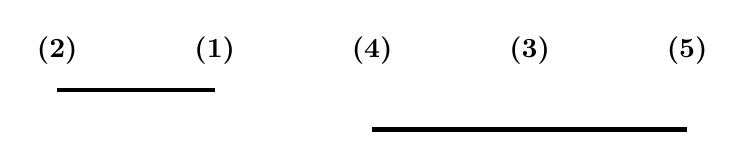
\begin{tikzpicture}[yscale=-1]
    % Define the positions of the labels
    \coordinate (2Pos) at (0, 0);
    \coordinate (1Pos) at (2, 0);
    \coordinate (4Pos) at (4, 0);
    \coordinate (3Pos) at (6, 0);
    \coordinate (5Pos) at (8, 0);
  
    % Draw the labels
    \node at (2Pos) {\textbf{(2)}};
    \node at (1Pos) {\textbf{(1)}};
    \node at (4Pos) {\textbf{(4)}};
    \node at (3Pos) {\textbf{(3)}};
    \node at (5Pos) {\textbf{(5)}};
  
    % Draw the line
    \draw[ultra thick] ([yshift=0.5cm]2Pos) -- ([yshift=0.5cm]1Pos);
    \draw[ultra thick] ([yshift=1cm]4Pos) -- ([yshift=1cm]5Pos);
  \end{tikzpicture}

  
  \noindent Treatments should be ordered from the smallest sample mean to the largest sample mean. This graph indicates that treatment 2 and 1 are not significantly different, and 4 and 3, and 5 are not significantly different.
\end{multicols}

\subsection*{Test of equality of variances}
\hrule width 6cm
\vspace{6pt}
Hypothesis: $H_0$: $\sigma_1^2 = \sigma_2^2 = \cdots = \sigma_a^2$. $H_a$: at least one $\sigma_i^2$ is different.
\paragraph{Bartlett's test} (use if data is normal) assumes normality for each treatment. Very sensitive to non-normality.
\paragraph{Modified Levene's test} (use if data $\approx$ normal) robust for non-normaility. For data from a normal dist, not as powerful as Bartlett's.


\section*{Conclusions}
\hrule width \textwidth
\vspace{6pt}
\paragraph{Rejection Methods} Reject $H_0$ if p-value $\leq \alpha$. Reject $H_0$ if the test statistic falls within the critical region.
\paragraph{$100(1-\alpha)\%$ C.I} "We are $100(1-\alpha)\%$ confident that the true \{test\} is between \{upper bound\} and \{lower bound\}."
\paragraph{Reject $H_0$} "There is enough statistical evidence to support (the statement of $H_a$)."
\paragraph{Fail to reject $H_0$} "There is not enough statistical evidence to support (the statement of $H_a$)."
or "The evidence from the data is consistent with (the statement of $H_0$)"


% \begin{figure}[h]
%   \centering
%   \begin{subfigure}[b]{0.3\textwidth}
%       \includegraphics[width=1.15\textwidth]{./images/a.png}
%     \label{fig:img1}
%   \end{subfigure}
%   \hfill
%   \begin{subfigure}[b]{0.3\textwidth}
%       \includegraphics[width=1.15\textwidth]{./images/b.png}
%     \label{fig:img2}
%   \end{subfigure}
%   \hfill
%   \begin{subfigure}[b]{0.3\textwidth}
%       \includegraphics[width=1.15\textwidth]{./images/c.png}
%     \label{fig:img2}
%   \end{subfigure}
%   \label{fig:both}
% \end{figure}

\end{document}
